% Filename: ForwardInverseToolkit.tex
% Last update: Thursday, September 7, 2017 by Ally Warner
%    - created
%
%%%%%%%%%%%%%%%%%%%%%%%%%%%%%%%%%%%%%%%%%%%%%%%%%%%%%%%%%%%%%%%%%%%%%%

\section{Methods}
\label{sec:Methods}

ADD PIPELINE FIGURE HERE

\subsection{Data Acquisition}
\label{sec:Data}

%%% Types of Images, Acquisition, and conversion

To construct a high-resolution, personalized, anisotropic volume conductor whole-head model, $T_1$-, $T_2$- weighted, diffusion weighted, and functional magnetic resonance (MRI) scans were acquired on a healthy, female volunteer who is 23 years of age on a Skyra 3T full-body scanner (Siemens Medical Solutions). The $T_1$-weighted scan was performed with a 3D magnetization prepared rapid gradient echo (MPRAGE) sequence (Mugler and Brookman, 1990) -- get this reference. The parameters used were as follows: echo time: 3.41ms, repetition time: 2500ms, flip angle: 7 $^{\circ}$, resolution matrix size: 256x256 pixels, field of view: 256mm, 208 sagittal slices with a slice thickness of 1mm. Acquisition time was 10:42 minutes. The $T_2$-weighted scan was performed with a sampling perfection with application-optimized contrast using different flip angle evolutions (check ref) (SPACE) sequence (Lichy et. al., 2005; Mugler et al., 2000). The parameters used were as follows: echo time: 406ms, repetition time: 3200ms, resolution matrix size: 256x256 pixels, field of view: 256mm, 208 sagittal slices with a slice thickness of 1mm. Acquisition time was 5:34 minutes. The subject did not move in between the two scans so the scans did not need to be registered. 

The diffusion weighted images (DWI) were acquired with multiband two-dimensional echo-planar imaging (EPI). Both phase encoding directions were performed (anterior to posterior and posterior to anterior) with 64 diffusion directions each. Further sequence parameters for each scan was as follows: echo time: 76.8ms, repetition time: 4070ms, flip angle: 90 $^{\circ}$, resolution matrix size: 104x104 pixels, field of view: 208mm, 60 slices with 2.5mm slice thickness. Acquisition time was 5:05 minutes. 

The function MRI (fMRI) scans were acquired with blood oxygenation level dependent contrast (BOLD). The following parameters were used:  echo time: 76.8ms, repetition time: 780ms, flip angle: 55 $^{\circ}$, resolution matrix size: 104x104 pixels, field of view: 210mm, 72 slices with 2mm slice thickness. Acquisition time was 10:32 minutes.

A continuous electroencephalogram (EEG) was recorded using a 256-channel HydroCel Geodesic Sensor Net that was connected to a NetAmps 400 amplifier and referenced online to a single vertex electrode. Channel impedances were kept at or below 50 kOhms and signals were sampled at 250Hz. The EEG was recorded while the subject sat quietly in a chair, alternating two minute epochs of eyes open and eyes closed for a total of 12 minutes. 

All acquisition reports will be included with the dataset. 

\subsection{Preprocessing of Images}
\label{sec:preprocess}

\subsubsection{MRI Correction}

Bias field signal is a low-frequency, smooth signal that corrupts MRI images due to inhomogeneities in the magnetic fields of the MRI machine by blurring images reducing the high frequencies of the images such as edges and contours. It changes the intensity values of image pixels so that the same tissue has a different distribution of grayscale intensities across the image. (ref) An estimated bias field correction on the $T_1$ and $T_2$ MRI's was done using FSL FAST.

(figure of the settings)

\subsubsection{DTI}

\begin{itemize}

\item DWI was preprocessed using DTIPrep which corrects for movement, badly acquired images, etc. 

\item DWI was converted to DTI using Slicer - (module) after registration.

\end{itemize}

\subsubsection{fMRI}

\begin{itemize}

\item fMRI was preprocessed using the fcon\_1000 pipeline. (specific to the University of Utah), includes registration to MRI

\end{itemize}


\subsubsection{Registration}

All scans were registered to the $T_1$ MRI. Since the subject did not move between the $T_1$ and $T_2$ MRIs, they did not need to be registered. However, the subject did move for the DWI. The cage (find proper name) was upgraded to the a higher resolution option. The subject did not move again for the fMRI. 

DWI and fMRI - manual registration using SCIRun

To register the DWI to the $T_1$ MRI, both scans must first be skull stripped which is to remove all tissues save for the brain. This was done using Brain Extraction Tool (BET2) in FMRIB Software Library (FSL). After the DWI was skull stripped, there was tissue remaining that was not part of the brain which was making the registration difficult. Both the $T_1$ MRI and the DWI were manually fixed using Seg3D by generating thresholding masks and erasing non-brain tissue. The DWI was registered to the $T_1$ MRI using 3D Slicer (ref) (www.slicer.org) with the skull stripped images with a rigid transform with six degrees of freedom. The 3D Slicer's linear registration transform output from registering the two brains was then applied to the full DWI image to register to the $T_1$ MRI. The fMRI was registered as described in a later section using the f\_con1000 pipeline. 

FIGURES

Give each software a small definition?

\subsection{MRI Segmentation of Tissues}
\label{sec:Seg}

%%% Preparation for segmentation, trials, manual work 

Segmentation of the head tissues proved to be the most time consuming section of the pipeline. The head volume was segmented into air, cerebral spinal fluid (CSF), white matter, grey matter, skull, sinus, eyes, and scalp. Segmentation of the brain can be difficult due to the similar intensities of the different tissues, making merely applying a median filter and thresholding the image not enough. (show a figure of this happening?)

The brain was initially segmented by inputing a skull stripped $T_1$ MRI into FSL FAST Segmentation. This outputs CSF, white matter, and grey matter layers as well as a bias-corrected $T_1$ MRI. This method, compared with Freesurfer, Statistical Parametric Mapping through Matlab (SPM), Atlas Based Classification through 3D Slicer, and Seg3D methods alone, produced the best initial brain segmentation results for this data due to how well it filled in each tissue. (??) (three panel figure of FSL FAST results)

Although the FSL Fast results were a great improvement compared to the other segmentation trials, manual segmentation still needed to be done on those layers to add more detail and take out any cross over between the layers. Since white matter is the innermost layer, it was worked on first. All manual editing was done using Seg3D software. (ref) First a threshold layer was created from the FSL Fast output. Every slice in every direction was inspected and manually edited whether that was adding more detail that could be seen with the naked eye or cleaning up noise from FSL Fast. This manual editing of the white matter took roughly 40 hours of work. (Figure of before and after editing -- hook detail!) 

After the white matter was completed, a threshold layer for grey matter was created from the FSL Fast output. Each slice in every direction of the grey matter was inspected as well. The white matter layer was removed from the grey matter using a boolean remove mask filter. Any holes between the two layers were decided manually. More detail was added to the grey matter folds to add to the CSF layer as well. The last part of editing the grey matter was decided to add a grey matter nucleus to the layer. The thresholding algorithms generated a lot of noise around these nuclei so they were segmented by hand, using the paintbrush tool, and added to the grey matter layer with a boolean or mask filter. The nuclei were also removed from the white matter layer using a boolean remove mask filter. The manual editing of the grey matter took roughly 20 hours of work. (figures of grey matter and nuclei)

After the grey and white matter layers were completed, the CSF layer was made by creating a solid threshold layer for the entire brain and removing the white and grey matter layers using a boolean remove mask filter. The white matter, grey matter, and CSF layers were then checked for holes, whether on the surface or the inside of the segmentation. Also a quality check on the layers was performed to ensure that the layers were at least two pixels wide. This is an important note for creating a hole-less tetrahedral mesh. The creation of the CSF layer and the manual editing and hole checking took roughly 4 hours of work. (??) (Figures of CSF? Figures of all three brain layers together?)

The skull and the sinus layers are the most difficult to segment using only an MRI because they both appear black in the image, and the volunteer did not have a CT scan. (define CT-scan) The first attempt to create a bone layer was first to use FSL's skull stripping using the BET2 tool to create a skull. Then to threshold the remainder of the bones in Seg3D from the $T_1$ MRI and connect it to the skull from FSL. (figure and compare the two skull layers) Although this gave a decent skull for only having an MRI layer, the method to segment sinus layer was still to be determined. As a second method, the skull was estimated from an MR-based synthetic pseudo-CT. An improved iterative version of the patch-based method was used described by Torrado-Carvajal et al. [ref] that takes the $T_1$ and $T_2$ images as input, and synthesize the pseudo-CT based on both images providing more refined and accurate bone boundaries. MR input images were preprocessed to correct for MRI bias inhomogeneities (N4 bias correction tool in the Insight Toolkit)(ref?) prior to computing the pseudo-CT. (figure of the pseudo-CT output) This method gave a good starting place for skull segmentation, but still needed manual editing. After using a median filter (pixel radius?) and thresholding, each slice in each direction was manually edited by hand. (figure of segmentation) Since the volunteer has a permanent retainer in their mouth, the mouth was segmented as solid bone for now. This is not concerning because the EEG cap used did not cover the volunteer's mouth. (picture? explain EEG caps) The pseduo-CT image also provided a segmentation of the sinuses and esophagus by thresholding the black pixels. After the thresholding, the sinus layer was also manually edited. Quality checks were done on both layers to ensure that there were no holes and that the layers were at least two pixels thick. (figure) Manually editing the second skull and the sinuses took roughly 30-40 hours of work. 

The eyes, skin, and air layers were simple, in comparison, to segment. The eyes were easily segmented by thresholding the $T_2$ MRI. (figure of T2 axially) The skin layer was segmented by thresholding the entire volume and removing all of the previous layers using a boolean remove mask filter. A quality check was performed on the skin layer to ensure that it was at least two pixels thick. The important places to check for this is at the bridge of the nose and the bottom of the chin. (sagittal figure) Last, the air was segmented by thresholding the entire image and removing the solid skin layer. (how much time?) There was a check to ensure that the segmentation did not contain any holes between layers after they were removed. (should I explain this procedure?) To create these three layers took roughly 8 hours of work, most of which was ensuring there were no holes in the segmentation. This is imperative to creating a quality mesh.

(Should I make a table instead for the amount of work?)

\subsection{Finite Element Mesh Generation}
\label{sec:mesh}

%%% Settings for mesh generation, issues 

The tetrahedral finite element mesh was generated using Cleaver software (ref and figure) on a Late 2013 Mac Pro with a 2.7 Ghz 12 Core Intel Xeon E5 processor, 64 GB of RAM, and an AMD FirePro graphics card. To make a very high resolution mesh with no holes the following parameters were used: scaling factor: 0.6, size multiplier: 1.0, lipschitz: 0.2, padding: 0, element sizing method: apdative. This produced a mesh with 60.2 million elements and 10.3 million nodes. (figure[s]) This mesh was so large due to the complexity of the segmentation. To reduce the size of the mesh, a mesh was made with a scaling factor of 1.0 with the remainder of the parameters as described before. The computing sizing field was exported from Cleaver and manipulated using SCIRun4 (ref and figure of network) by.... changing the scaling by 27??...The changed sizing field was then input into Cleaver and cleaved a new mesh. This produced a mesh with 15.7 million elements and 2.7 million nodes with no holes. However, this mesh does contain one flat tetrahedra. It is later removed in a SCIRun network, and is currently being investigated by Cleaver software developers. To reduce the size of the mesh even further, to be able to use on smaller machines, mesh simplification was considered via MeshLab (ref and figure). FIGURE THIS OUT. 

\section{Conductivity Preparation}

All conductivities were homogeneous with the exception of white matter when using DTI tensor data. These conductivities are as follows: ADD HERE (ref). When DTI tensor data is added, there are two approaches to converting the tensor data to conductivities. The first is scaling the data, and the second is giving the white matter a fixed ratio of conductivity. 

SCALING MATH (ref)

RATIO MATH (ref)

\subsection{Mathematical Modeling}
\label{sec:math}

%%%

\subsection{Numerical Methods}
\label{sec:numerical}

%%%

\subsection{Simulations}
\label{sec:Sims}

%%%SCIRun networks

\begin{itemize}

\item Forward problem 

\item Include figures of SCIRun networks - how much detail??

\end{itemize}

END OF ALLY'S TEXT

\subsubsection{Experimental Methods}
\label{sec:ExpMethods}

%%% This paragraph addresses the Experimental Preparation
We induced episodes of acute, transient ischemia  in anesthetized, open-chest swine (n = ??) and 
canine (n = ??) preparations. In each experiment, the heart was exposed and suspended in a 
pericardial cradle.  A portion of the LAD was minimally dissected and fitted with  a hydraulic occluder, 
which could be compressed to restrict coronary blood flow, thereby creating the transient ischemic 
condition, and then released to restore normal cardiac perfusion.  Experimental protocols consisted of 
measuring extracellular potentials, both on the epicardial surface and within the myocardium, while 
applying stepwise increases of ischemic load \cite{RSM:Ara2014}.  To this end, two basic protocols 
were used to induce ischemia: 1) LAD blood flow was incrementally reduced by the occluder while 
maintaining a constant, often elevated, heart rate (supply ischemia) or 2) increases in the heart rate 
were applied while maintaining a constant, often restricted, LAD blood flow (demand ischemia).  For 
purposes of this study, we do not consider the differences between supply and demand ischemia but 
rather focus on the size, shape, and location of the zones within the heart that show an electrical 
response to the ischemic condition.    All studies were performed in accordance with the Guide for the 
Care and Use of Laboratory Animals (NIH Pub. No 85-23, Revised 1996).

%%% This paragraph addresses the data acquisition
Customized sock and needle electrodes were used to acquire electrical recordings of both epicardial 
and intramural electrical potentials.  A 247-electrode, flexible sock array,\cite{RSM:Ari92} with recording electrodes 
evenly distributed across the ventricles, acquired epicardial electrogram recordings. Twenty-five (25) 
flexible fiberglass plunge needles\cite{RSM:Rog2002} were used to record intramural electrical activity. Plunge needles 
were constructed with 10 evenly spaced electrodes at 1.6 mm intervals along the shaft.  Needles 
were placed in and around the perfusion bed of the occluded LAD.  Sock and needle recordings were 
made periodically at a 1KHz sampling rate, the combination of which provided a \emph{3-dimensional} 
electrical representation of the induced ischemic condition.

%%% This paragraph addresses geometric set-up to be more fully covered later
In addition to the acquisition of electrical recordings, digitized locations of sock electrodes and needle 
locations were extracted for postexperiment validation studies. After digitization, needle electrodes 
were removed and replaced with radio-opaque spacers prior to cardiac imaging in order to provide a 
registration reference.

%%% This paragraph addresses Post-experiment Data Processing
Electrograms were calibrated, gain adjusted, and baseline corrected against control recordings, which 
had been taken immediately before each intervention. Poor quality electrograms, caused by broken lead 
connections or bad contacts, as well as electrograms without positive Q-wave deflections (identified as 
cavity electrodes) were discarded. The global root mean squared signal was computed from data 
recordings of both sock and needle electrodes.  These signals were used to identify a point that lay at 
40\% of the distance between the J point and T wave peak (ST40\%).  Potential difference maps were 
generated at ST40\%, which compared baseline recordings to those obtained during an ischemic 
episode.  Potential differences, taken at ST40\% during baseline conditions, were used to generate a threshold by which ischemic regions were identified as values exceeding two standard deviations.
Sock recordings were used to validate simulation findings and will be addressed later.  Needle 
electrodes were used to generate subject-specific ischemic zone geometries by identifying regions
within a spatial neighborhood that met the above-mentioned ischemic thresholding criteria.\cite{RSM:Ara2009}

\subsection{Simulation Pipeline}
\label{sec:Pipeline}

%%%%%%%%%%%%%%%%
% Fix this figure with the text and images that Rob wanted to see in previous email
%%%%%%%%%%%%%%%%
\begin{figure}[h!]
\centering
%    \includegraphics[width=\textwidth]{Figures/Simulation_Pipeline.pdf}
    \includegraphics[width=\textwidth]{Figures/Simulation_Pipeline_Flat.pdf}    
    \caption{\label{fig:pipeline} Ischemia Simulation Pipeline. Both image and time signals were extracted from experimental protocols of acute, induced ischemic preparations.  Image data was used to generate geometries through segmentation and meshing.  Intramural electrical data, recorded from plunge needles, were mapped to these meshes to define ischemic zone location.  New meshes were generated with ischemic geometries imposed on which ischemic simulations were generated and validated against the original experimental data recorded from epicardial sock data.}
\end{figure}
%% Replace pipeline with a more linear representation (Josh's suggestion)

%%%Move Imaging to the center, flatten other sections of pipeline
A simulation pipeline was implemented in order to produce in silico models that were representative of 
experimental findings. Electrical data acquired during the experimental process, as well as imaging 
information acquired post experiment, were used to construct subject-specific, finite element, bioelectric simulations by way of the steps illustrated in Figure \ref{fig:pipeline}.

\subsubsection{Imaging and Segmentation}
%%% This paragraph addresses imaging and segmentation -- The beginning of the sim pipeline image
After completion of the experimental protocol, each heart was excised and scanned with a 7 tesla MRI 
scanner using FISP and FLASH MRI sequences.  Diffusion tensor images (DTI) were also acquired to 
determine fiber direction.  FISP scans rendered consistent, albeit low, contrast throughout the tissue - 
preserving edges near the field of view boundaries.  FLASH scans, in comparison, provided images of 
high contrast within the center of the volume, which diminished steeply near the field of view 
boundaries.  The advantages of both FISP and FLASH were combined in order to produce realistic, 
geometric segmentations of blood, cardiac tissue, and needles,  using the Seg3D\footnote{http://sci.utah.edu/software.html} open-source
software package. Needle locations were readily identified within the scans as  dark regions 
occupied by the radio-opaque spacers that were inserted at the end of the experimental phase.  
Diffusion-weighted MRI (DW-MRI) images were also obtained from which fiber orientation was derived.  


\subsubsection{Geometric Processing and Data Mapping}
\label{ssec:geom}

%%% This paragraph addresses meshing
Segmentations were used to generate realistic \emph{3-dimensional} geometries for use in subsequent finite element simulations (See Section \ref{ssec:FEM}).  By using two open-source meshing 
packages, we were able to generate smooth, linear, subject-specific, boundary-conforming, tetrahedral 
meshes for use in simulations. First, segmentations were ported into the BioMesh3D\footnotemark[1] software package 
% This may need to be altered if either BioMesh or Cleaver is removed from the pipeline
to generate smoothed/tightened surface representations.  BioMesh3D surface representations were 
used as input indicator functions to a second meshing package, Cleaver\footnotemark[1], from which the final mesh was 
derived.  Cleaver is a multimaterial meshing package that produces structured meshes of tetrahedral 
elements with guaranteed minimum element angles,\cite{SCI:Bro2014a} resulting in quality meshes that require fewer computational resources.  Cleaver, however, does not offer the surface-tightening features of 
BioMesh3D.  As a result, meshes produced by Cleaver from standard MRI segmentations (with no 
surface tightening) would propagate the stair-stepped surfaces inherent in rasterized, volumetric data.  
By combining packages, we were able to produce smooth, structured meshes of guaranteed element 
quality.

%%% This paragraph addresses needle registration and data mapping to the mesh
Correspondence points derived from known sock and needle locations were used to register needle and sock electrode geometries within the cardiac mesh using the SCIRun problem-solving environment
\footnotemark.  Processed data values were mapped to corresponding node locations within the cardiac 
mesh. Linear interpolation to local nodes was applied but restricted to the geometric convex hull of the 
needle locations.  Extrapolation to outlying regions, not within the scope of needle locations, was not 
included. % DOUBLECHECK Double check the linear interpolation step...If radial basis is used, this statement is incorrect

%%% This paragraph addresses ischemic zone identification within the mesh
To identify ischemic zones, potential difference maps were generated that removed baseline potentials from those observed during ischemic interventions.  Difference map values within the specified needle region that exceeded a value greater than two standard deviations from baseline 
recordings were identified and labeled as ischemic.  These new label masks 
were used to create a final mesh that contained three defined tissues (blood, healthy cardiac tissue, 
and ischemic cardiac tissue) that shared conforming surfaces - an important feature in static forward 
simulations when considering areas in proximity to potential sources.\cite{SCI:Swe2010a}

%%% This paragraph addresses fiber mapping
Finally, subject-specific fiber orientation was applied within the mesh. A vector 
field was defined by the principle eigenvector from DW-MRI images with all other cross-sectional fiber 
components regarded as isotropic. This vector field was normalized, aligned, and mapped to the cardiac 
mesh using weighted-average interpolation to provide a basis for anisotropic conductivity. 

\subsubsection{Mathematical Modeling}
%%% This paragraph addresses the Bidomain (should I mention Laplace�s, or more accurately Poisson�s, equation here)
The cardiac mesh, with associated fiber structure and ischemic region, was used to solve the 
bidomain passive current flow equation:
\begin{equation}
\nabla \cdot (\bar{\sigma}_e + \bar{\sigma}_i)\nabla \phi_e = - \nabla \cdot \bar{\sigma}_i \nabla V_m
\label{eq:bidomain}
\end{equation}
where $\sigma_e$ and $\sigma_i$ represent the extracellular and intracellular conductivity tensors, 
respectively.  $\phi_e$ is the extracellular potentials, and $V_m$ represents the transmembrane 
potential. 

%%% These paragraphs address parameters used for the simulations (BC,\sigma,Vm, BZ)
� � � � � � � �%Boundary conditions
In this model, it was assumed that the heart was surrounded by a perfect insulator, leading to a 
Neumann boundary condition on the epicardial surface.  The endocardium, in contrast, allowed for 
extracellular, but not intracellular, current flow into the ventricular blood pool. Initial blood potentials 
were defined by Cauchy boundary conditions along the endocardial surface as shown in Equation 
\ref{eq:initial}. % possibly site MacLachlan 2005 % DOUBLECHECK: model may be Neumann conditions in the blood as well...follow up after the model is finalized.  Also, if we do use both Neumann and Dirichlet, these are Cauchy boundary conditions.
\[   
   \begin{cases} 
      \nabla \cdot (\bar{\sigma}_e + \bar{\sigma}_i)\nabla \phi_e = - \nabla \cdot \bar{\sigma}_i V_m & x \in \Omega_H\\
      \vec{n}_{epi} \cdot (\bar{\sigma}_e + \bar{\sigma}_i)\nabla \phi_e = 0 & x \in \partial\Omega_{H,epi} \\
      %\vec{n}_{endo} \cdot (\bar{\sigma}_i \nabla \phi_i) = 0 & x \in \partial\Omega_{H,endo} \\      
      \vec{n}_{endo} \cdot (\bar{\sigma}_e \nabla \phi_e) = -\vec{n}_{b} \cdot (\bar{\sigma}_b \nabla \phi_b) & x \in \partial\Omega_{H,endo} \\         
      \phi_e = \phi_b & x \in \partial\Omega_{H,endo} \\
      \phi_i = 0 & x \in \Omega_{b} 
      \label{eq:initial}
   \end{cases}
   \numberthis
\]  
where $\Omega_H$ represents the cardiac volume; $\partial\Omega_{H,epi}$ and $\partial
\Omega_{H,endo}$ the epicardial and endocardial surfaces, respectively;  $\phi_e$ and $\phi_b$ 
correspond to potentials in the extracellular space and the blood, respectively. $\vec{n}$ represents 
the normal, outward unit vector along the epicardial ($epi$), endocardial ($endo$), and blood ($b$) 
surfaces.  The first equation specifies the relationship between transmembrane and extracellular 
potentials within the cardiac domain. The following four equations define the handling of currents and 
potentials along the cardiac surfaces.  The blood, in all studies, was completely enclosed within the cardiac 
region  and considered to have isotropic conductivity (See Figure \ref{fig:heartschematic} and Table 
\ref{tab:cond}).

%� � � � � � � �Conductivities
\begin{figure}[!th]
    \centering
    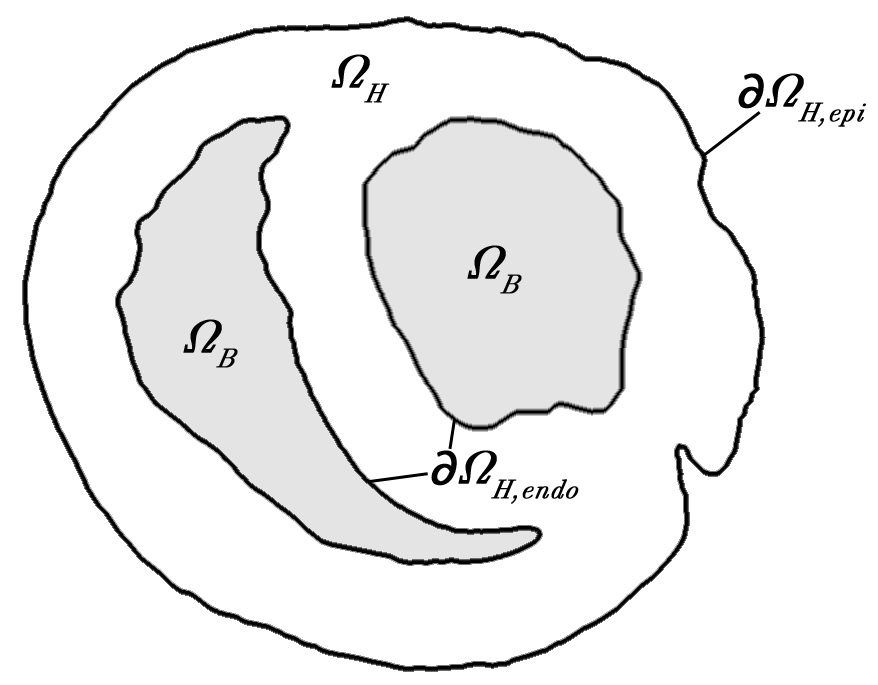
\includegraphics[width=9cm]{Figures/HeartRegions.jpg}
    \caption{Bidomain equations are defined within the cardiac tissue $\Omega_H$ and bounded by epicardial and endocardial boundaries $\Omega_{H,epi}$ and $\Omega_{H,endo}$. Extracellular currents were allowed to flow into the blood volume $\Omega_{B}$ along the endocardial boundary. }
    \label{fig:heartschematic}
\end{figure}

Conductivity values within the tissue, as well as the blood pool, were normalized with respect to 
extracellular longitudinal values and matched those used in previous studies.\cite{RSM:Hop2004,BMB:Swe2010a,SCI:Sti2003a} Table 
\ref{tab:cond} shows the conductivity values used for this study.  These conductivity values were 
chosen to be consistent with those previously defined by Johnston and Kilpatrick \cite{BMB:Joh2003}. % DOUBLECHECK...Bruce's thesis points to the Johnston study, but the actual paper does not seem to use these same values.
Conductivities within the ischemic region were reduced with respect to healthy values corresponding 
to the first 5 - 15 minutes after ischemic onset. %also cite Circulation, 60 (1979), pp. 397�403 && m J Cardiol 1984;53:307-312 On desktop, read and add to BMB DOUBLECHECK 10-15 minutes here

\begin{table}[t]
    \caption{\label{tab:cond}Ratio applied to tensor conductivity values
      within healthy and ischemic regions. \cite{RSM:Hop2004}} 
    \vspace{4 mm}
    \centerline{\begin{tabular}{ccc} \hline\hline
          \specialcell{Conductivity \\ Labels}   & \specialcell{Healthy \\ Conductivity Values} & \specialcell{Ischemic \\ Conductivity Values} \\ \hline
          $\sigma_{el}$   & 1 & 1/2 \\
          $\sigma_{il}$   & 1 & 1 \\
          $\sigma_{et}$  & 1/3 & 1/4 \\
          $\sigma_{it}$  & 1/20 & 1/20 \\ 
          $\sigma_{b}$  & 3 & 3 \\ \hline\hline
      \end{tabular}}
\end{table}

We defined a fixed transmembrane potential value ($V_m$) of 30mV as the potential source for our 
forward simulations.  The reduced transmembrane potential mimics the delayed activation of diseased 
tissue under ischemic conditions during the ST-segment.
Healthy tissue was assigned a value of 0 mV, typical of the relatively quiescent state of healthy cardiac 
activation during the ST segment.  Between healthy and ischemic tissue, a border zone was defined in 
which potentials progressed from the diseased to healthy states.

The border zone, the region between healthy and ischemic tissue, has been determined to be a necessary, 
and problematic, region to include in simulation studies.\cite{BMB:Swe2010a,RSM:Hop2004,BMB:Kil2003} 
In this study, we defined the border zone as a piecewise, continuous function represented by Equation \ref{eq:border} in which a Gaussian function defines the region from the ischemic zone boundary 
to a specified transition point, $S_1$.  At $S_1$ the border transitions to a linear, decreasing function 
that reduces to $0$ (the value assigned to healthy tissue) at $S_2$.   It is important to note that not all 
models, found in the literature, have applied border zones.  For the sake of consistency and uniformity, 
however, we have imposed border regions into all of the forward simulations constructed in this paper.  
Table \ref{tab:BZvals} shows the values applied to Equation \ref{eq:border} for this study.

\[    BZ = 
   \begin{cases} 
      V_m e^{\frac{-d^2}{2\sigma^2}} & d < S_1\\
      \Gamma - \frac{\Gamma}{S_2 - S_1}(d-S_1) & S_1 \leq d < S_2 \\
      0 & d \geq S_2
   \end{cases}
      \numberthis
      \label{eq:border}
\]
\begin{center}
where
$\Gamma = V_m e^{\frac{-(S_1)^2}{2\sigma^2}} $
\end{center}

\begin{table}[h]
    \caption{\label{tab:BZvals}Values Used In Border Zone Determination.} 
    \vspace{4 mm}
    \centerline{\begin{tabular}{ccc} \hline\hline
          \specialcell{Label}   & \specialcell{Definition} & \specialcell{Value} \\ \hline
          $V_m$   & Transmembrane Potential  & 30 mV \\
          $\sigma$   & Gaussian RMS Width  & 5 mm \\ %double check
          $S_1$  & First Transition Distance  & 8 mm \\
          $S_2$  & Second Transition Distance  & 11 mm \\ 
          $d$  & $distance$ & $variable$ \\ \hline\hline
      \end{tabular}}
\end{table}

\subsubsection{Numerical Methods}
\label{ssec:FEM}
%%% This paragraph addresses Finite Element Discretization

Solutions to Equation \ref{eq:bidomain} were computed using finite element methods.  By applying 
Green's divergence theorem to Equation \ref{eq:bidomain}, the following weak formulation is generated 
\begin{equation}
\int ((\bar{\sigma}_e + \bar{\sigma}_i)\nabla \phi_e) \cdot \nabla \psi(\bar{x})d\bar{x} = - \int (\bar{\sigma}
_i \nabla V_m)\cdot \nabla \psi(\bar{x})d\bar{x}, \quad \quad \forall \ \psi \in \Omega
\label{eq:galerkin}
\end{equation}
where, $\Omega$ (see Section Section \ref{ssec:geom}) is the linear, finite element mesh, $\psi$ 
represents the finite element basis functions characterized by local hat functions associated with 
mesh nodes.  By applying this formulation to the finite dimensional mesh, we can reduce Equation 
\ref{eq:galerkin} to a system of linear equations 
\begin{equation}
A \phi_e = -RV_m
\label{eq:ReducedFormula}
\end{equation}
where $A$ and $R$ represent stiffness matrices defined by $A_{j,k} = \langle \nabla \psi_j,(\bar{\sigma}
_e + \bar{\sigma}_i)\nabla \psi_k \rangle_\Omega$ and $R_{j,k} = \langle \nabla \psi_j,\bar{\sigma}_i
\nabla \psi_k \rangle_\Omega$,
while $\phi_e$ and $V_m$ represent extracellular and transmembrane potentials, respectively.\cite{BMB:Wan2013}

%%% This paragraph addresses SCIRun as a solver
We used the open-source, SCIRun problem solving environment\cite{BMB:Par95} to apply parameters and 
to solve Equation  \ref{eq:ReducedFormula} numerically.  Within the SCIRun environment, fiber orientation 
and conductivity tensors were applied to the  mesh, initial and boundary conditions were defined, and 
border regions were generated in order to compute extracellular potentials by way of a conjugate gradient 
method with a Jacobi preconditioner.

\subsubsection{Comparison Approaches}
Epicardial potentials compared using CC, RMS Error, and DICE correlation...Do it first, then explain it.

\subsubsection{Validation}
%%% This paragraph addresses sock registration and data mapping to the mesh 
In order to validate solutions of the ischemic condition, experimental data was compared to simulated 
solutions.  Experimental data were mapped to the mesh by digitizing and later registering sock electrodes to points identified on the surface of the cardiac mesh.  Potential data from sock electrodes were interpolated onto the ventricular surfaces and compared to simulated potentials on a node-to-node correspondence.  RMS error and the correlation coefficient between simulated epicardial potentials and experimental sock data were generated to assess accuracy of simulation results.



%\subsubsection{Comparison models}
%%% This paragraph highlights other ischemic zone representations (lots of refs)
% rough writing
%Similar to the us of FISP and FLASH MRI modalities to derive subject-specific cardiac geome
%%% This paragraph outlines the system for comparing current vs. subject specific zones
% rough writing
%Similar to the us of FISP and FLASH MRI modalities to derive subject-specific cardiac geome

%\subsection{Methods subsection}
%\label{sec:methodssub}
%
%A methods  subsection, Section~\ref{sec:methodssub}
%
%\subsubsection{A methods subsubsection}
%\label{sec:methodssubsub}
%
%And a subsubsection, Section~\ref{sec:methodssubsub}.


